% Gray Code in 4-cube
% Author: Yury Chebiryak <http://yury.chebiryak.name/index.html>
\documentclass[a3paper,landscape]{article}
\usepackage{tikz}
%%%<
\usepackage{verbatim}
%\usepackage[active,tightpage]{preview}
%\PreviewEnvironment{tikzpicture}
%\setlength\PreviewBorder{5pt}%
%%%>

\begin{comment}
:Title: Gray Code in 4-cube

Depicts a Gray code traversing all the nodes of a 4-dimensional hypercube. See `<http://yury.chebiryak.name/hypercubes.htm>`_ for more details.

\end{comment}
\begin{document}
\pagestyle{empty}
\begin{center}
 \begin{figure}[bt]
 \centering
 \scalebox{0.6}
 {
 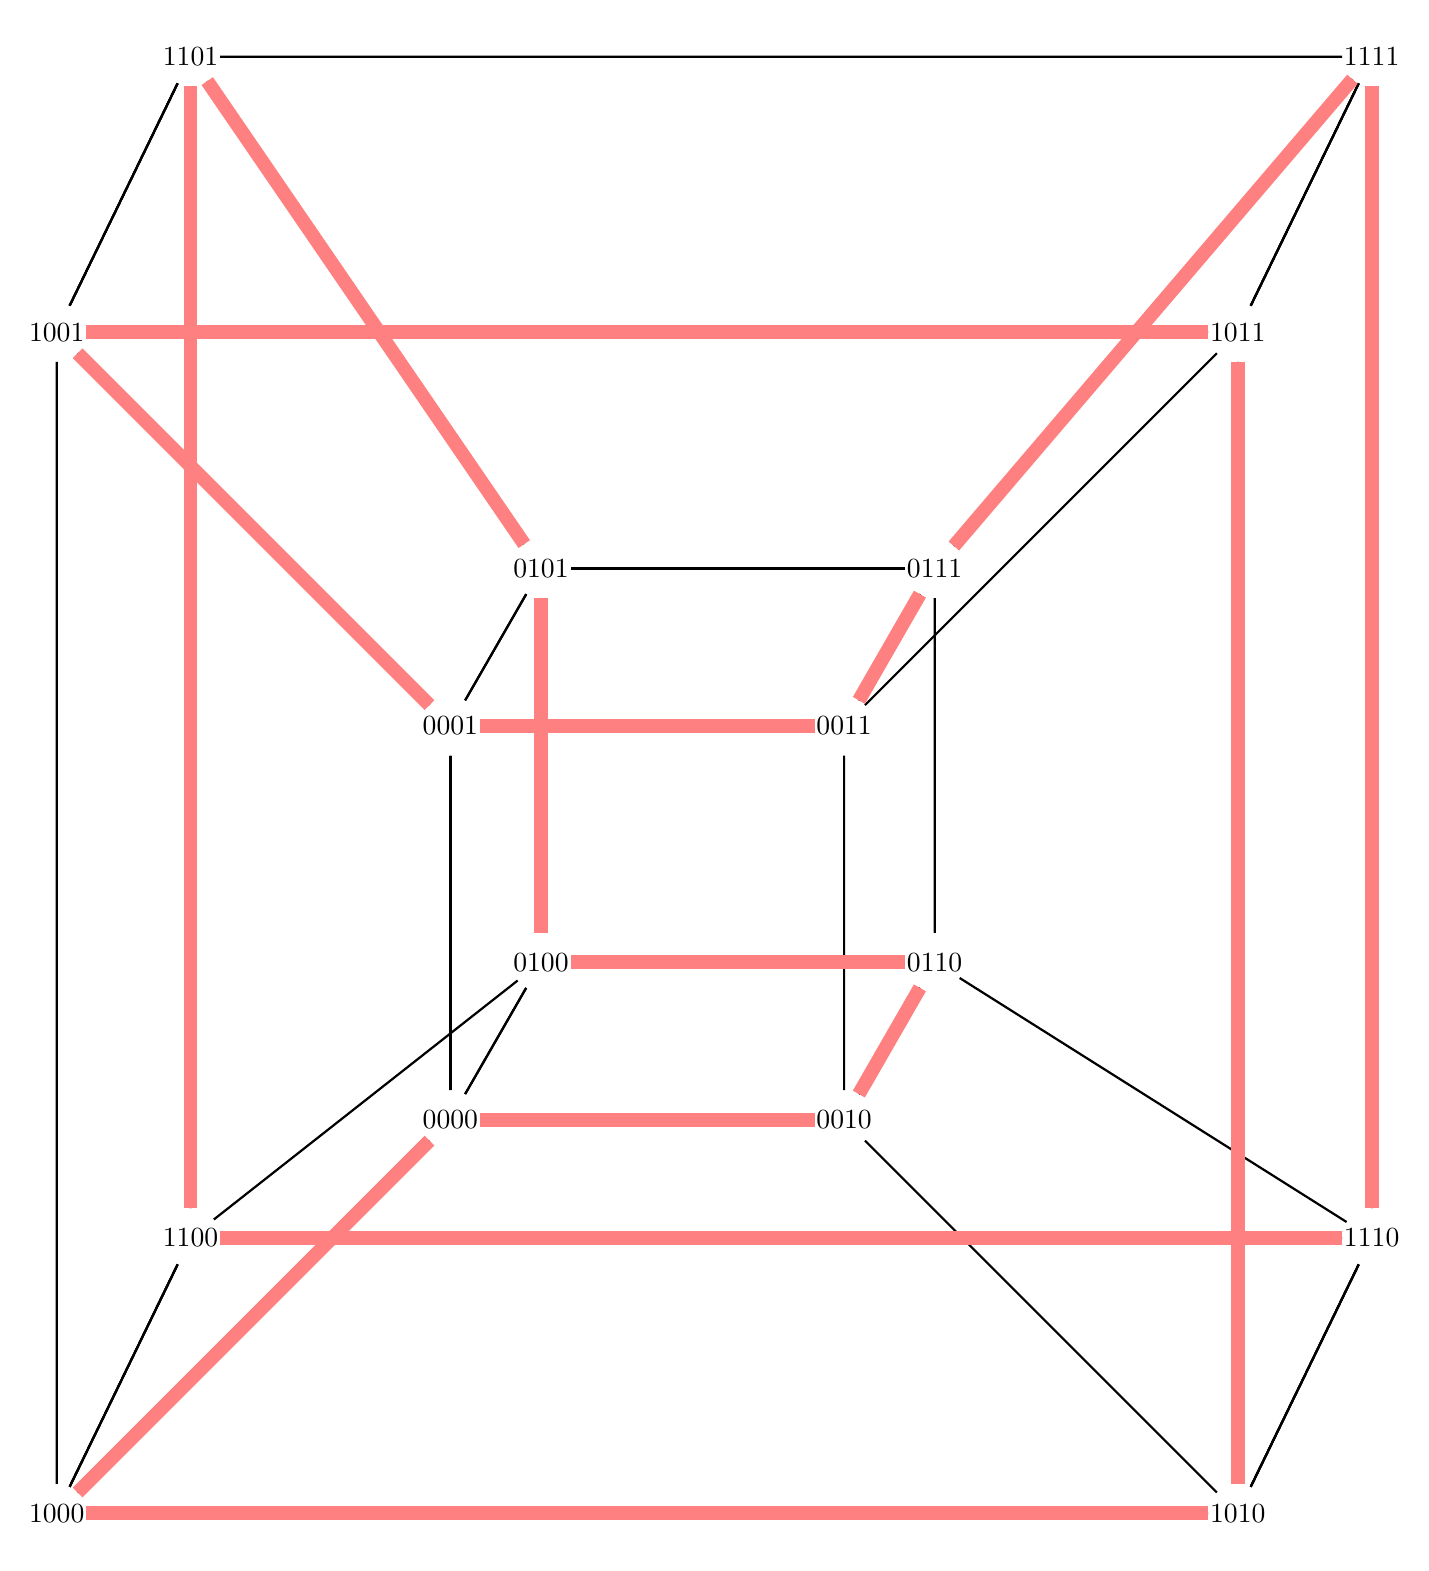
\begin{tikzpicture}[scale=5]
	 \tikzstyle{vertex}=[circle,minimum size=20pt,inner sep=0pt]
	 \tikzstyle{selected vertex} = [vertex, fill=red!24]
	 \tikzstyle{selected edge} = [draw,line width=5pt,-,red!50]
	 \tikzstyle{edge} = [draw,thick,-,black]
	 \node[vertex] (v0) at (0,0) {$0000$};
	 \node[vertex] (v1) at (0,1) {$0001$};
	 \node[vertex] (v2) at (1,0) {$0010$};
	 \node[vertex] (v3) at (1,1) {$0011$};
	 \node[vertex] (v4) at (0.23, 0.4) {$0100$};
	 \node[vertex] (v5) at (0.23,1.4) {$0101$};
	 \node[vertex] (v6) at (1.23,0.4) {$0110$};
	 \node[vertex] (v7) at (1.23,1.4) {$0111$};
	 \node[vertex] (v8) at (-1,-1) {$1000$};
	 \node[vertex] (v9) at (-1,2) {$1001$};
	 \node[vertex] (v13) at (-0.66,2.7) {$1101$};
	 \node[vertex] (v12) at (-0.66,-0.3) {$1100$};
	 \node[vertex] (v10) at (2,-1) {$1010$};
	 \node[vertex] (v14) at (2.34,-0.3) {$1110$};
	 \node[vertex] (v11) at (2,2) {$1011$};
	 \node[vertex] (v15) at (2.34,2.7) {$1111$};
	 \draw[edge] (v0) -- (v1) -- (v3) -- (v2) -- (v0);
	 \draw[edge] (v0) -- (v4) -- (v5) -- (v1) -- (v0);
	 \draw[edge] (v2) -- (v6) -- (v7) -- (v3) -- (v2);
	 \draw[edge] (v4) -- (v6) -- (v7) -- (v5) -- (v4);
	 \draw[edge] (v8) -- (v9) -- (v13) -- (v12) -- (v8);
	 \draw[edge] (v0) -- (v4) -- (v12) -- (v8) -- (v0);
	 \draw[edge] (v1) -- (v9) -- (v13) -- (v5) -- (v1);
	 \draw[edge] (v2) -- (v10) -- (v14) -- (v6) -- (v2);
	 \draw[edge] (v8) -- (v10) -- (v14) -- (v12) -- (v8);
	 \draw[edge] (v3) -- (v11) -- (v15) -- (v7) -- (v3);
	 \draw[edge] (v10) -- (v11) -- (v15) -- (v14) -- (v10);
	 \draw[edge] (v9) -- (v11) -- (v15) -- (v13) -- (v9);
	 \draw[selected edge] (v0) -- (v2);
	 \draw[selected edge] (v2) -- (v6);
	 \draw[selected edge] (v6) -- (v4);
	 \draw[selected edge] (v4) -- (v5);
	 \draw[selected edge] (v5) -- (v13);
	 \draw[selected edge] (v13) -- (v12);
	 \draw[selected edge] (v12) -- (v14);
	 \draw[selected edge] (v14) -- (v15);
	 \draw[selected edge] (v15) -- (v7);
	 \draw[selected edge] (v7) -- (v3);
	 \draw[selected edge] (v3) -- (v1);
	 \draw[selected edge] (v1) -- (v9);
	 \draw[selected edge] (v9) -- (v11);
	 \draw[selected edge] (v11) -- (v10);
	 \draw[selected edge] (v10) -- (v8);
	 \draw[selected edge] (v8) -- (v0);
 \end{tikzpicture}
 }
 \caption{Complete Gray Code}
 \end{figure}
 \end{center}
\end{document}
